\documentclass[aspectratio=169,10pt]{beamer}

% ─────────────────────────────────────────────────────────────
%  THEME & COLOUR SETUP
% ─────────────────────────────────────────────────────────────
\usetheme{Madrid}
\usecolortheme{default}

% Custom deep-blue / gold palette
\definecolor{deepblue}{RGB}{10,36,82}       % dominant dark navy
\definecolor{midblue}{RGB}{30,80,160}       % secondary blue
\definecolor{accentgold}{RGB}{205,160,40}   % accent gold
\definecolor{lightgray}{RGB}{240,242,246}   % slide background tint
\definecolor{textdark}{RGB}{20,20,40}       % body text

% Apply colours to beamer elements
\setbeamercolor{palette primary}{bg=deepblue,fg=white}
\setbeamercolor{palette secondary}{bg=midblue,fg=white}
\setbeamercolor{palette tertiary}{bg=deepblue,fg=white}
\setbeamercolor{palette quaternary}{bg=deepblue,fg=white}
\setbeamercolor{structure}{fg=deepblue}
\setbeamercolor{section in toc}{fg=deepblue}
\setbeamercolor{frametitle}{bg=deepblue,fg=white}
\setbeamercolor{title}{bg=deepblue,fg=white}
\setbeamercolor{block title}{bg=midblue,fg=white}
\setbeamercolor{block body}{bg=lightgray,fg=textdark}
\setbeamercolor{block title alerted}{bg=accentgold,fg=deepblue}
\setbeamercolor{block body alerted}{bg=accentgold!15,fg=textdark}
\setbeamercolor{block title example}{bg=deepblue!70,fg=white}
\setbeamercolor{block body example}{bg=deepblue!8,fg=textdark}
\setbeamercolor{item}{fg=deepblue}
\setbeamercolor{subitem}{fg=midblue}

% ─────────────────────────────────────────────────────────────
%  FONTS
% ─────────────────────────────────────────────────────────────
\usefonttheme{professionalfonts}
\setbeamerfont{title}{size=\large,series=\bfseries}
\setbeamerfont{frametitle}{size=\normalsize,series=\bfseries}
\setbeamerfont{block title}{size=\small,series=\bfseries}

% ─────────────────────────────────────────────────────────────
%  INNER THEME — rounded corners, numbered circles
% ─────────────────────────────────────────────────────────────
\useinnertheme{rounded}
\setbeamertemplate{enumerate items}[circle]
\setbeamertemplate{itemize items}[circle]
\setbeamertemplate{navigation symbols}{}   % remove nav bar

% Footer
\setbeamertemplate{footline}{%
  \leavevmode%
  \hbox{%
    \begin{beamercolorbox}[wd=.33\paperwidth,ht=2.4ex,dp=1ex,center]{palette secondary}%
      \usebeamerfont{author in head/foot}\insertshortauthor
    \end{beamercolorbox}%
    \begin{beamercolorbox}[wd=.34\paperwidth,ht=2.4ex,dp=1ex,center]{palette primary}%
      \usebeamerfont{title in head/foot}\insertshorttitle
    \end{beamercolorbox}%
    \begin{beamercolorbox}[wd=.33\paperwidth,ht=2.4ex,dp=1ex,center]{palette secondary}%
      \usebeamerfont{date in head/foot}%
      \insertframenumber{} / \inserttotalframenumber
    \end{beamercolorbox}%
  }%
}

% ─────────────────────────────────────────────────────────────
%  PACKAGES
% ─────────────────────────────────────────────────────────────
\usepackage{amsmath,amssymb,amsfonts}
\usepackage{mathtools}
\usepackage{bm}
\usepackage{algorithm}
\usepackage{algpseudocode}
\usepackage{booktabs}
\usepackage{array}
\usepackage{xcolor}
\usepackage{graphicx}
\usepackage{tikz}
\usetikzlibrary{arrows.meta, positioning, shapes.geometric, backgrounds}
\usepackage{tcolorbox}
\tcbuselibrary{skins,theorems}

% ─────────────────────────────────────────────────────────────
%  CUSTOM COMMANDS
% ─────────────────────────────────────────────────────────────
\newcommand{\C}{\mathbb{C}}
\newcommand{\R}{\mathbb{R}}
\newcommand{\Z}{\mathbb{Z}}
\newcommand{\calH}{\mathcal{H}}
\newcommand{\calN}{\mathcal{N}}
\newcommand{\calL}{\mathcal{L}}
\newcommand{\calS}{\mathcal{S}}
\newcommand{\tensor}{\otimes}
\newcommand{\Tr}{\mathrm{Tr}}

% Highlighted equation box
\tcbset{
  eqbox/.style={
    enhanced, colback=midblue!8, colframe=midblue,
    boxrule=0.6pt, arc=3pt, left=4pt, right=4pt,
    top=2pt, bottom=2pt, fonttitle=\bfseries\footnotesize,
    attach boxed title to top left={yshift=-1.5mm,xshift=3mm},
    boxed title style={colback=midblue,arc=2pt}
  },
  keyresult/.style={
    enhanced, colback=accentgold!12, colframe=accentgold!80!black,
    boxrule=0.8pt, arc=4pt, left=5pt, right=5pt,
    top=3pt, bottom=3pt
  }
}

% ─────────────────────────────────────────────────────────────
%  TITLE INFORMATION
% ─────────────────────────────────────────────────────────────
\title[Quantum Comm.\ Framework]{%
  Rigorous Quantum Communication Framework\\
  for Electromagnetic Signals in Optical Fibres}

\subtitle{Cq Channel Capacity $\cdot$ Noisy Channel Analysis $\cdot$
  Integrated Control $\cdot$ Computational Hardness}

\author[Kaumud Sharma]{%
  \textbf{Kaumud Sharma}\\[2pt]
  {\small Quantum Communication Theory Group}}

\date{February 2026 \quad$\cdot$\quad Internship Report, Weeks~1--4}

% ═══════════════════════════════════════════════════════════════
\begin{document}
% ═══════════════════════════════════════════════════════════════

% ────────────────────────────── TITLE SLIDE ──────────────────
{%
\setbeamertemplate{footline}{}
\begin{frame}[plain]
  \titlepage
\end{frame}
}

% ──────────────────────────── OUTLINE ────────────────────────
\begin{frame}{Outline}
  \tableofcontents[
    sectionstyle=show,
    subsectionstyle=show/shaded,
    subsubsectionstyle=hide
  ]
\end{frame}

% ═══════════════════════════════════════════════════════════════
\section{Week 1: Physical Foundations and Cq Channel Framework}
% ═══════════════════════════════════════════════════════════════

% ───────────────────── MOTIVATION ────────────────────────────
\begin{frame}{Motivation and Key Distinctions}
\begin{columns}[T]
  \column{0.48\textwidth}
    \textbf{Classical vs.\ Quantum Communication}\\[6pt]
    Classical channels: abstract $p(y|x)$.\\
    Quantum optical fibres: three critical distinctions:
    \medskip
    \begin{enumerate}
      \item \textbf{Quantum nature of light}\\
            {\small Creation/annihilation operators, not amplitudes.}
      \item \textbf{Non-commutative measurements}\\
            {\small Homodyne vs.\ heterodyne vs.\ photon counting.}
      \item \textbf{Physical parameter dependence}\\
            {\small $n_{\text{core}},n_{\text{clad}},a,\beta_2,\alpha,L$.}
    \end{enumerate}

  \column{0.48\textwidth}
    \begin{block}{Holevo Bound}
      \vspace{2pt}
      \[
        I(X{:}Y)\;\le\;\chi\bigl(\{p(x),\rho(x)\}\bigr)
        = S(\bar\rho)-\sum_x p(x)\,S(\rho(x))
      \]
      \vspace{-2pt}
      {\small $\bar\rho=\sum_x p(x)\rho(x)$;\quad
        $S(\rho)=-\Tr[\rho\log\rho]$ (von~Neumann entropy)}
    \end{block}
    \medskip
    \begin{alertblock}{Goal}
      Develop a complete, rigorous framework from Maxwell's equations
      to computational hardness of decoding.
    \end{alertblock}
\end{columns}
\end{frame}

% ─────────────────── MAXWELL + FIBRE ─────────────────────────
\begin{frame}{Electromagnetic Field Propagation in Optical Fibres}
\begin{columns}[T]
  \column{0.50\textwidth}
    \textbf{Maxwell's Equations} (inhomogeneous medium):
    \begin{align*}
      \nabla\cdot\mathbf{D}&=\rho_{\text{free}},\quad
      \nabla\cdot\mathbf{B}=0,\\
      \nabla\times\mathbf{E}&=-\tfrac{\partial\mathbf{B}}{\partial t},\quad
      \nabla\times\mathbf{H}=\mathbf{J}+\tfrac{\partial\mathbf{D}}{\partial t}.
    \end{align*}

    \textbf{Step-index fibre:}
    \[
      n(r)=\begin{cases}n_{\text{core}},&r<a,\\n_{\text{clad}},&r>a.\end{cases}
    \]

    \textbf{Key parameters:}
    \[
      \text{NA}=\sqrt{n_{\text{core}}^2-n_{\text{clad}}^2},\quad
      V=\frac{2\pi a}{\lambda_0}\,\text{NA}
    \]
    Single-mode condition: $V<2.405$.

  \column{0.46\textwidth}
    \begin{block}{Gaussian Pulse Propagation}
      \[
        A(t,z)=\frac{A_0}{\sqrt{1-i\beta_2 z/T_0^2}}
        \exp\!\left(-\frac{(t-\beta_1 z)^2}{2T_0^2(1-i\beta_2 z/T_0^2)}\right)
      \]
      Pulse width: $T(z)=T_0\sqrt{1+(z/L_D)^2}$\\
      Dispersion length: $L_D=T_0^2/|\beta_2|$\\[4pt]
      Attenuation: $P(z)=P(0)\,e^{-2\alpha_{\text{Np}}z}$
    \end{block}

    \begin{exampleblock}{LP$_{01}$ Mode Profile}
      \[
        \mathbf{E}_{01}(r)\propto
        \begin{cases}J_0(ur/a), & r<a,\\
        \frac{J_0(u)}{K_0(w)}K_0(wr/a), & r>a.\end{cases}
      \]
    \end{exampleblock}
\end{columns}
\end{frame}

% ─────────────────── QUANTISATION ────────────────────────────
\begin{frame}{Quantum Field Theory in Optical Fibres}
\begin{columns}[T]
  \column{0.50\textwidth}
    \textbf{Field Quantisation:}
    \begin{align*}
      \hat{\mathbf{A}}(\mathbf{r},t)&=\sum_m
      \sqrt{\frac{\hbar\omega_m}{2\epsilon_0\epsilon_m V_m}}
      \bigl[\hat{a}_m f_m(\mathbf{r})+\hat{a}_m^\dagger f_m^*(\mathbf{r})\bigr]
    \end{align*}
    Commutation: $[\hat{a}_m,\hat{a}_n^\dagger]=\delta_{mn}$

    \medskip
    \textbf{Field Hamiltonian:}
    \[
      \hat{H}_{\text{field}}=\sum_m\hbar\omega_m
      \!\left(\hat{a}_m^\dagger\hat{a}_m+\tfrac{1}{2}\right)
    \]

    \textbf{Coherent state propagation:}
    \[
      \alpha(L)=\alpha(0)\,e^{i\beta(\omega)L}\,e^{-\alpha L/2}
    \]
    \[
      \hat\rho(L)=|\alpha(L)\rangle\langle\alpha(L)|
    \]

  \column{0.46\textwidth}
    \begin{block}{Atom-Field Coupling (RWA)}
      \[
        g(\theta)=d_{eg}\sqrt{\frac{\omega_0^3}
        {2\hbar\epsilon_0 V_{\text{eff}}(\theta)}}\,
        |f_0(\mathbf{r}_{\text{atom}}|\theta)|
      \]
      with $V_{\text{eff}}(\theta)\sim\pi a^2 L_{\text{eff}}$.
    \end{block}
    \medskip
    \begin{block}{Master Equation with Dissipation}
      {\small
      \[
        \frac{d\hat\rho}{dt}=-\frac{i}{\hbar}[H,\hat\rho]
        +\gamma\!\left(\sigma_-\hat\rho\sigma_+
        -\tfrac{1}{2}\{\sigma_+\sigma_-,\hat\rho\}\right)
        +\kappa\!\left(\hat a\hat\rho\hat a^\dagger
        -\tfrac{1}{2}\{\hat a^\dagger\hat a,\hat\rho\}\right)
      \]
      }
    \end{block}
\end{columns}
\end{frame}

% ─────────────────── CQ CHANNEL ──────────────────────────────
\begin{frame}{Classical-Quantum (Cq) Channel Theory}
\begin{columns}[T]
  \column{0.50\textwidth}
    \textbf{Cq Channel Definition:}
    \[
      W:\mathcal{X}\to\mathcal{S}(\mathcal{H}),\quad
      x\mapsto\rho(x|\theta)
    \]

    \textbf{Holevo Quantity:}
    \[
      \chi\bigl(\{p(x),\rho(x|\theta)\}\bigr)
      =S(\bar\rho)-\sum_x p(x)\,S(\rho(x|\theta))
    \]

    \begin{alertblock}{Channel Capacity}
      \[
        C(\theta)=\max_{p(x)}\chi\bigl(\{p(x),\rho(x|\theta)\}\bigr)
      \]
    \end{alertblock}

  \column{0.46\textwidth}
    \begin{block}{BPSK Example}
      $\mathcal{X}=\{0,1\}$, coherent-state encoding:
      \begin{align*}
        x{=}0&:\;\rho(0|\theta)=|\alpha(\theta)\rangle\langle\alpha(\theta)|\\
        x{=}1&:\;\rho(1|\theta)=|-\alpha(\theta)\rangle\langle{-}\alpha(\theta)|
      \end{align*}
      \[
        \alpha(\theta)=\alpha_0\,e^{i\beta(\theta)L}\,e^{-\alpha(\theta)L/2}
      \]
    \end{block}
    \medskip
    \begin{exampleblock}{$N$-symbol Transmission}
      \[
        \rho(x_1,\dots,x_N|\theta)=
        \bigotimes_{k=1}^N\rho(x_k|\theta)
      \]
      Naive MAP complexity: $\mathcal{O}(M^N\cdot d^2)$
    \end{exampleblock}
\end{columns}
\end{frame}

% ─────────────────── NP-HARDNESS INTRO ───────────────────────
\begin{frame}{NP-Hardness of Optimal Decoding (SJIP)}
  \begin{columns}[T]
    \column{0.50\textwidth}
      \begin{block}{Definition: SJIP}
        Given a semigroup $(G,\circ)$, element $y\in G$, and finite set
        $S\subseteq G$:\\[4pt]
        \emph{Does there exist $S'\subseteq S$ such that
        $\prod_{x\in S'}x=y$?}
      \end{block}
      \medskip
      \begin{alertblock}{Theorem (NP-Hardness)}
        SJIP is NP-hard via polynomial-time reduction from
        \textsc{Subset-Sum}.
      \end{alertblock}
      \medskip
      \textbf{Proof sketch:}
      \begin{itemize}
        \item Let $G=(\Z,+)$, $S=A$, $y=T$.
        \item $\exists S'\subseteq A:\sum a_i=T\iff$ SJIP has a solution.
        \item Reduction runs in $\mathcal{O}(n)$ time.
        \item $\Rightarrow\;\textsc{Subset-Sum}\le_p\textsc{SJIP}$.
      \end{itemize}

    \column{0.46\textwidth}
      \begin{exampleblock}{Consequence}
        Optimal decoding for a coherent-state Cq channel in optical
        fibres is \textbf{at least as hard as SJIP} — and therefore
        \textbf{NP-hard}.
      \end{exampleblock}
      \bigskip

      % Simple complexity comparison diagram
      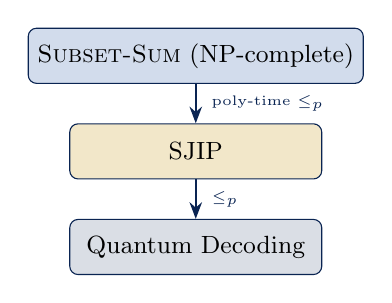
\begin{tikzpicture}[font=\small,
          box/.style={draw=deepblue,fill=lightgray,rounded corners=3pt,
                      minimum width=3.2cm,minimum height=0.7cm,align=center}]
        \node[box,fill=midblue!20] (ss) {\textsc{Subset-Sum} (NP-complete)};
        \node[box,below=0.5cm of ss,fill=accentgold!25] (sjip) {SJIP};
        \node[box,below=0.5cm of sjip,fill=deepblue!15] (dec) {Quantum Decoding};
        \draw[-{Stealth[length=6pt]},thick,deepblue]
          (ss) -- node[right,xshift=2pt]{\tiny poly-time $\le_p$} (sjip);
        \draw[-{Stealth[length=6pt]},thick,deepblue]
          (sjip) -- node[right,xshift=2pt]{\tiny $\le_p$} (dec);
      \end{tikzpicture}
  \end{columns}
\end{frame}

% ═══════════════════════════════════════════════════════════════
\section{Week 2: Noisy Quantum Channels}
% ═══════════════════════════════════════════════════════════════

% ─────────────────── GKSL ────────────────────────────────────
\begin{frame}{GKSL Master Equation and Fibre Noise Sources}
\begin{columns}[T]
  \column{0.50\textwidth}
    \textbf{Two primary noise sources:}
    \medskip
    \begin{enumerate}
      \item \textbf{Amplitude damping} (photon loss):
      \[
        \gamma_{\text{loss}}=\frac{\alpha v_g\ln10}{10}
      \]
      \item \textbf{Phase damping} (dephasing):
      \[
        \gamma_\varphi=\frac{(\omega D_p\Delta L)^2 v_g}{2}
      \]
    \end{enumerate}

    \medskip
    \textbf{Amplitude-damping Kraus operators:}
    \[
      E_0=\begin{pmatrix}1&0\\0&\sqrt{1-\eta}\end{pmatrix},\quad
      E_1=\begin{pmatrix}0&\sqrt{\eta}\\0&0\end{pmatrix}
    \]
    where $\eta(t)=1-e^{-\gamma_{\text{loss}}t}$.

  \column{0.46\textwidth}
    \begin{block}{GKSL Master Equation}
      \begin{align*}
        \frac{d\rho_S}{dt}&=-i[H_S,\rho_S]\\
        &\quad+\sum_k\gamma_k\!\left(L_k\rho_S L_k^\dagger
        -\tfrac{1}{2}\{L_k^\dagger L_k,\rho_S\}\right)
      \end{align*}
    \end{block}
    \medskip
    \begin{exampleblock}{Exact Solution Methods}
      \begin{itemize}
        \item \textbf{Direct:} $\vec\rho(t)=e^{\mathcal{L}t}\vec\rho(0)$,
          cost $\mathcal{O}(d^6)$.
        \item \textbf{Quantum trajectory method} (non-Markovian):
        \[
          \dot{|\psi\rangle}=-iH_{\text{eff}}|\psi\rangle
          +\sum_k\xi_k(t)L_k|\psi(t{-}\tau_k)\rangle
        \]
      \end{itemize}
    \end{exampleblock}
\end{columns}
\end{frame}

% ─────────────────── CAPACITY BOUNDS ─────────────────────────
\begin{frame}{Holevo Capacity for Noisy Channels}
\begin{columns}[T]
  \column{0.50\textwidth}
    \begin{block}{Noisy Channel Capacity}
      \[
        C_\chi(\mathcal{N})=\max_{\{p(x),\rho_x\}}
        \chi\bigl(\{p(x),\mathcal{N}(\rho_x)\}\bigr)
      \]
    \end{block}
    \medskip
    \textbf{Depolarising channel:}
    \[
      \mathcal{N}_{\text{dep}}(\rho)=(1{-}p)\rho+p\,\mathbf{I}/d
    \]
    \[
      C_\chi^{\text{dep}}=1-H_2\!\left(\tfrac{p}{2}\right)-p\log_2 3
    \]
    \medskip
    \textbf{Fibre noise channel:}
    \[
      C_\chi^{\text{fibre}}\le
      \min\!\bigl\{C_\chi^{\text{AD}}(\gamma),\,
      C_\chi^{\text{PD}}(\lambda)\bigr\}
    \]

  \column{0.46\textwidth}
    \begin{alertblock}{Quantum Data Processing Inequality}
      For Markov chain $\rho\to\sigma\to\tau$:
      \[
        I(\rho;\tau)\le I(\rho;\sigma)
      \]
    \end{alertblock}
    \medskip
    \begin{alertblock}{Capacity Non-Increase (CPTP)}
      For any quantum channel $\mathcal{N}$ and CPTP map $\mathcal{C}$:
      \[
        C_\chi(\mathcal{C}\circ\mathcal{N})\le C_\chi(\mathcal{N})
      \]
      \textbf{Corollary:} Post-channel CPTP correction
      \emph{cannot} increase capacity.
    \end{alertblock}
\end{columns}
\end{frame}

% ─────────────────── NON-INJECTIVITY ─────────────────────────
\begin{frame}{Decoding Ambiguity and Channel Non-Injectivity}
\begin{columns}[T]
  \column{0.50\textwidth}
    \begin{block}{Channel Non-Injectivity}
      For any non-unitary channel $\mathcal{N}$, $\exists$ distinct
      states $\rho_1\ne\rho_2$ such that
      \[
        \mathcal{N}(\rho_1)=\mathcal{N}(\rho_2).
      \]
    \end{block}
    \medskip
    \textbf{Ambiguity set:}
    \[
      \mathcal{A}(\sigma)=\bigl\{\rho'\in\mathcal{D}(\mathcal{H}_A)
      :\mathcal{N}(\rho')=\sigma\bigr\}
    \]

    \begin{alertblock}{Capacity-Ambiguity Trade-off}
      \[
        C_\chi(\mathcal{N})\le\log_2\!\left(\frac{1}{A_{\min}}\right)
      \]
      where $A_{\min}$ is the minimum achievable ambiguity.
    \end{alertblock}

  \column{0.46\textwidth}
    \medskip
    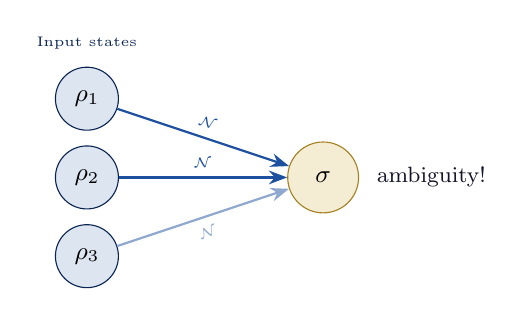
\begin{tikzpicture}[font=\small,
        state/.style={circle,draw=deepblue,fill=midblue!15,
                      minimum size=0.8cm,inner sep=1pt},
        output/.style={circle,draw=accentgold!80!black,fill=accentgold!20,
                       minimum size=0.9cm,inner sep=1pt}]
      \node[state] (r1) at (0,1.5) {$\rho_1$};
      \node[state] (r2) at (0,0.5) {$\rho_2$};
      \node[state] (r3) at (0,-0.5) {$\rho_3$};
      \node[output] (s) at (3,0.5) {$\sigma$};
      \node[right=0.1cm of s,text=textdark] {\footnotesize ambiguity!};
      \draw[-{Stealth},thick,midblue] (r1) -- (s)
        node[above,sloped,midway,font=\tiny]{$\mathcal{N}$};
      \draw[-{Stealth},thick,midblue] (r2) -- (s)
        node[above,sloped,midway,font=\tiny]{$\mathcal{N}$};
      \draw[-{Stealth},thick,midblue!50] (r3) -- (s)
        node[below,sloped,midway,font=\tiny]{$\mathcal{N}$};
      \node[above=0.1cm of r1,font=\tiny,text=deepblue]{Input states};
    \end{tikzpicture}

    \medskip
    \textbf{Key insight:} Noise-induced non-injectivity creates
    \emph{information-theoretic} ambiguity, which stacks on top of the
    \emph{computational} hardness of SJIP.
\end{columns}
\end{frame}

% ═══════════════════════════════════════════════════════════════
\section{Week 3: Integrated Quantum Control and SJIP Proof}
% ═══════════════════════════════════════════════════════════════

% ─────────────────── CONTROLLED DYNAMICS ─────────────────────
\begin{frame}{Integrated Quantum Control During Channel Evolution}
\begin{columns}
  \column{0.50\textwidth}
    \textbf{Uncontrolled dynamics:}
    \[
      \frac{d\rho}{dt}=\mathcal{L}_0(\rho)=
      -i[H_0,\rho]+\sum_{k=1}^2\gamma_k\!\left(L_k\rho L_k^\dagger
      -\tfrac{1}{2}\{L_k^\dagger L_k,\rho\}\right)
    \]

    \textbf{With control Hamiltonian $H_c(t)$:}
    \[
      \frac{d\rho}{dt}=\bigl(\mathcal{L}_0+\mathcal{L}_c(t)\bigr)(\rho),
      \quad\mathcal{L}_c(t)(\rho)=-i[H_c(t),\rho]
    \]
    \[
      [\mathcal{L}_0,\mathcal{L}_c(t)]\ne0\quad
      \text{(essential for noise suppression)}
    \]

    \begin{alertblock}{Key: TPCP Theorem}
      The controlled map $\mathcal{S}_t(\rho(0))=
      \mathcal{T}\!\exp\!\bigl(\int_0^t(\mathcal{L}_0+\mathcal{L}_c)\,d\tau\bigr)\rho(0)$
      is trace-preserving and completely positive for all $t\ge0$.
    \end{alertblock}

  \column{0.46\textwidth}
    \begin{block}{Capacity Enhancement Theorem}
      Let $f_k(t)\in[0,1]$ be suppression factors. Controlled
      efficiency:
      \[
        \eta_c(t)=\exp\!\!\left(-\gamma_1\int_0^t f_1(\tau)\,d\tau\right)
      \]
      If $\int_0^t f_1\,d\tau<t$ then
      \[
        \boxed{C_\chi(\mathcal{S}_t)>C_\chi(\mathcal{N}_t)}
      \]
      because $C$ is strictly increasing in $\eta$.
    \end{block}
\end{columns}
\end{frame}

% ─────────────────── CONTROL MECHANISMS ──────────────────────
\begin{frame}{Practical Control Mechanisms}
  \begin{columns}[T]
    \column{0.32\textwidth}
      \begin{block}{Dynamical Decoupling}
        $\pi$-pulse sequence:
        \[
          H_c(t)=\sum_n\pi\delta(t{-}n\tau)\sigma_x
        \]
        \[
          \gamma_\varphi^{\text{eff}}=
          \gamma_\varphi\cdot\text{sinc}^2(\omega\tau)\to0
        \]
        as $\tau\to0$.
      \end{block}

    \column{0.32\textwidth}
      \begin{block}{Quantum Error Correction}
        For a $[[n,k,d]]$ code:
        \[
          \gamma_1^{\text{eff}}=\gamma_1\binom{n}{t}p^t(1{-}p)^{n-t}
        \]
        where $t=\lfloor(d{-}1)/2\rfloor$.
      \end{block}

    \column{0.32\textwidth}
      \begin{block}{Hamiltonian Engineering}
        Design $H_c(t)$ satisfying:
        \begin{itemize}
          \item $[H_c,H_{\text{signal}}]=0$\\
            {\tiny (preserves information)}
          \item $\{H_c,L_k\}\propto0$\\
            {\tiny (suppresses noise)}
        \end{itemize}
      \end{block}
  \end{columns}

  \bigskip
  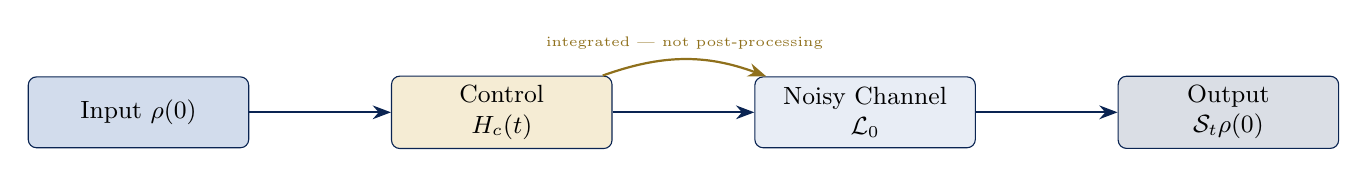
\begin{tikzpicture}[font=\small,
      node distance=1.8cm,
      box/.style={draw=deepblue,fill=lightgray,rounded corners=3pt,
                  minimum width=2.8cm,minimum height=0.9cm,align=center}]
    \node[box,fill=midblue!20] (in) {Input $\rho(0)$};
    \node[box,right=of in,fill=accentgold!20] (ctrl) {Control\\$H_c(t)$};
    \node[box,right=of ctrl,fill=midblue!10] (ch) {Noisy Channel\\$\mathcal{L}_0$};
    \node[box,right=of ch,fill=deepblue!15] (out) {Output\\$\mathcal{S}_t\rho(0)$};
    \draw[-{Stealth},thick,deepblue] (in) -- (ctrl);
    \draw[-{Stealth},thick,deepblue] (ctrl) -- (ch);
    \draw[-{Stealth},thick,deepblue] (ch) -- (out);
    \draw[-{Stealth},thick,accentgold!70!black,bend left=20]
      (ctrl) edge node[above,font=\tiny]{integrated — not post-processing} (ch);
  \end{tikzpicture}
\end{frame}

% ─────────────────── SJIP FULL PROOF ─────────────────────────
\begin{frame}{Rigorous SJIP NP-Hardness Proof}
\begin{columns}[T]
  \column{0.50\textwidth}
    \textbf{Setup:} Quadratic semigroup
    $\mathcal{F}=\{f_a(z)=(z+a)^2:a\in\Z\}$
    under function composition.

    \smallskip
    \textbf{Composition law:}
    $f_a\circ f_b(z)=((z+b)^2+a)^2$

    \medskip
    \textbf{Inversion ambiguity:}
    Given $f_{a_i}(z_{i-1})=z_i$:
    \[
      z_{i-1}=\epsilon_i\sqrt{z_i}-a_i,\quad
      \epsilon_i\in\{\pm1\}
    \]

    \begin{alertblock}{Lemma}
      $\exists S'\subseteq A:\sum_{a_i\in S'}a_i=T$ \textbf{iff}
      $\exists\;\boldsymbol\epsilon\in\{\pm1\}^n$ such that backward
      iteration from $z_n=T^2$ yields $z_0=0$.
    \end{alertblock}

  \column{0.46\textwidth}
    \begin{block}{Theorem: $\textsc{Subset-Sum}\le_p\textsc{SJIP}$}
      \textbf{Multiplicative version:}\\
      $G=(\C,\times)$,\; $S=\{e^{a_i}\}$,\; $y=e^T$.
      \[
        \prod_{a_i\in S'}e^{a_i}=e^T\iff\sum_{a_i\in S'}a_i=T
      \]
      \smallskip
      \textbf{Time:} $\mathcal{O}(n)$ arithmetic operations.
    \end{block}
    \medskip
    \begin{alertblock}{Corollary}
      If a poly-time algorithm for SJIP exists $\Rightarrow P=NP$.
    \end{alertblock}
\end{columns}
\end{frame}

% ═══════════════════════════════════════════════════════════════
\section{Week 4: Channel Estimation, Comparison and Security}
% ═══════════════════════════════════════════════════════════════

% ─────────────────── QFIM & QCRB ─────────────────────────────
\begin{frame}{Quantum Fisher Information and Cramér--Rao Bound}
\begin{columns}[T]
  \column{0.50\textwidth}
    \textbf{Symmetric Logarithmic Derivative (SLD):}
    \[
      \partial_\mu\rho_\Theta=
      \tfrac{1}{2}(\rho_\Theta L_\mu+L_\mu\rho_\Theta)
    \]
    \[
      L_\mu=\!\sum_{\substack{i,j\\\lambda_i+\lambda_j>0}}
      \!\!\frac{2\langle e_i|\partial_\mu\rho|e_j\rangle}
      {\lambda_i+\lambda_j}\,|e_i\rangle\langle e_j|
    \]

    \textbf{Quantum Fisher Information Matrix (QFIM):}
    \[
      F_{\mu\nu}(\Theta)=\mathrm{Re}\,\Tr[\rho_\Theta L_\mu L_\nu]
    \]

    \begin{alertblock}{Quantum Cramér--Rao Bound}
      For any locally unbiased estimator $\hat\Theta$ from $M$ copies:
      \[
        \mathrm{Cov}_\Theta(\hat\Theta)\ge\frac{1}{M}\,F(\Theta)^{-1}
      \]
    \end{alertblock}

  \column{0.46\textwidth}
    \begin{block}{QFIM for Loss + Dephasing Channel}
      With $\eta=e^{-\gamma_{\text{loss}}L}$:
      \[
        F_{\mu\nu}=
        \begin{pmatrix}
          \frac{1}{\eta\bar n}+\frac{4\gamma_\varphi^2 L^2}{\eta\bar n}
          & 0\\[6pt]
          0 & 4\eta\bar n\,e^{-2\gamma_\varphi L}
        \end{pmatrix}
      \]
      $+\;\mathcal{O}(\bar n^{-2})$
    \end{block}
    \medskip
    \begin{block}{Adaptive Strategy (LAN)}
      \[
        \lim_{M\to\infty}M\cdot\mathrm{Cov}(\hat\Theta_M)
        =F(\Theta_0)^{-1}
      \]
      The bound is \textbf{asymptotically achievable} via local
      asymptotic normality (LAN).
    \end{block}
\end{columns}
\end{frame}

% ─────────────────── THREE PARADIGMS ─────────────────────────
\begin{frame}{Comparative Analysis: Three Decoding Paradigms}
  \begin{columns}[T]
    \column{0.32\textwidth}
      \begin{block}{Paradigm 1\\Uncontrolled}
        \[
          \hat x=\arg\max_x\Tr[\Pi_y\rho(x|\theta)]
        \]
        Complexity: $\mathcal{O}(M^N d^2)$\\[4pt]
        Rate $R_1$: baseline
      \end{block}

    \column{0.32\textwidth}
      \begin{block}{Paradigm 2\\CPTP-Corrected}
        \[
          \hat x=\arg\max_x\Tr[\Pi_y\mathcal{C}(\mathcal{N}(\rho))]
        \]
        By Data Processing:
        \[
          C_\chi(\mathcal{C}\circ\mathcal{N})\le C_\chi(\mathcal{N})
        \]
        Rate $R_2\le R_1$
      \end{block}

    \column{0.32\textwidth}
      \begin{alertblock}{Paradigm 3\\Controlled}
        \[
          \hat x=\arg\max_x\Tr[\Pi_y\mathcal{S}_t(\rho)]
        \]
        $\mathcal{S}_t=\mathcal{T}\exp\int(\mathcal{L}_0+\mathcal{L}_c)d\tau$\\[4pt]
        Rate $R_3>R_1$ (optimal control)
      \end{alertblock}
  \end{columns}

  \bigskip
  \begin{alertblock}{Complexity-Performance Trade-off Theorem}
    A decoding algorithm achieving $R\ge R_{\text{controlled}}-\varepsilon$
    with complexity $\mathcal{O}(\mathrm{poly}(N,M,1/\varepsilon))$ exists
    \textbf{if and only if} $NP\subseteq BQP$.
  \end{alertblock}
\end{frame}

% ─────────────────── SECURITY ────────────────────────────────
\begin{frame}{SJIP-Based Security and Noise-Assisted Cryptography}
\begin{columns}[T]
  \column{0.50\textwidth}
    \textbf{Eavesdropper's advantage:}
    \[
      \mathrm{Adv}(E)=\max_{\{\Pi_y\},D}
      \Pr[\hat x=x]-\frac{1}{|\mathcal{X}^N|}
    \]

    \begin{block}{SJIP-Based Security Theorem}
      If $NP\not\subseteq BQP$, for SJIP-based encoding:
      \[
        \mathrm{Adv}(E)\le\mathrm{negl}(N)
      \]
    \end{block}

    \begin{alertblock}{Noise Amplifies Security}
      For combined amplitude + phase damping:
      \[
        \mathrm{Adv}_{\text{noisy}}(E)\le
        \mathrm{Adv}_{\text{noiseless}}(E)
        \cdot e^{-\gamma_{\text{loss}}L}
        \cdot e^{-2\gamma_\varphi L}
      \]
    \end{alertblock}

  \column{0.46\textwidth}
    \begin{exampleblock}{Dual Security Layers}
      \[
        \Pr[\text{Eve succeeds}]\le
        \underbrace{\frac{1}{|\mathcal{A}(\sigma)|}}_{\text{info-theoretic}}
        +\underbrace{\mathrm{negl}(N)}_{\text{computational}}
      \]
    \end{exampleblock}
    \medskip

    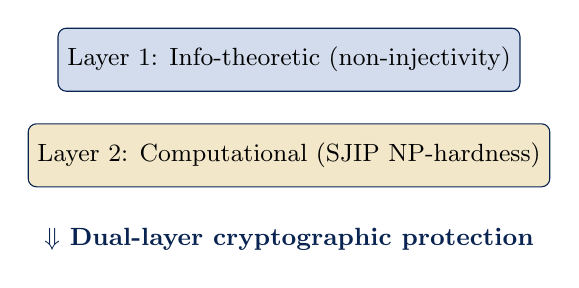
\begin{tikzpicture}[font=\small,
        layer/.style={draw=deepblue,fill=lightgray,rounded corners=3pt,
                      minimum width=4.2cm,minimum height=0.8cm,align=center}]
      \node[layer,fill=midblue!20] (l1)
        {Layer 1: Info-theoretic (non-injectivity)};
      \node[layer,below=0.4cm of l1,fill=accentgold!25] (l2)
        {Layer 2: Computational (SJIP NP-hardness)};
      \node[below=0.4cm of l2,text=deepblue,font=\bfseries\small]
        {$\Downarrow$ Dual-layer cryptographic protection};
    \end{tikzpicture}
\end{columns}
\end{frame}

% ─────────────────── ESTIMATION ALGORITHM ────────────────────
\begin{frame}{Channel Parameter Estimation Protocol}
\begin{columns}[T]
  \column{0.52\textwidth}
    \begin{block}{Algorithm: Adaptive Bayesian Estimation}
      \begin{algorithmic}[1]
        \footnotesize
        \Require Fibre sample, $M$ copies, prior $p_0(\Theta)$
        \Ensure $\hat\Theta$, confidence intervals
        \State Init $k=0$, $p_k(\Theta)=p_0(\Theta)$
        \While{$k<M$}
          \State $\bar F=\int F(\Theta)p_k(\Theta)\,d\Theta$
          \State Choose POVM maximising $\Tr[\bar F^{-1}F_\Pi(\Theta)]$
          \State Apply POVM, obtain $y_{k+1}$
          \State Update posterior $p_{k+1}$
          \State $k\leftarrow k+1$
        \EndWhile
        \State $\hat\Theta=\int\Theta\,p_M(\Theta)\,d\Theta$
        \Return $\hat\Theta$, covariance
      \end{algorithmic}
    \end{block}

  \column{0.44\textwidth}
    \textbf{Testable predictions:}
    \begin{enumerate}
      \item \textbf{Capacity scaling:}
        \[
          C(L,a,T)=C_0 e^{-\alpha L}(1{-}e^{-\kappa/a^2})
          (1{-}\gamma_T(T{-}T_0))
        \]
      \item \textbf{Noise rates:}
        $\gamma_{\text{loss}}=\frac{\alpha v_g\ln10}{10}$
      \item \textbf{Control gain:}
        \[
          \frac{\Delta C}{C}=1-e^{-\gamma_{\text{loss}}
          \int_0^L(1-f)d\tau}
        \]
      \item \textbf{Hardness signature:}
        Optimal $\sim\mathcal{O}(2^{\alpha N})$
        vs.\ approx $\sim\mathcal{O}(N^2)$
    \end{enumerate}
\end{columns}
\end{frame}

% ═══════════════════════════════════════════════════════════════
\section{Integrated Framework and Conclusion}
% ═══════════════════════════════════════════════════════════════

% ─────────────────── SUMMARY TABLE ───────────────────────────
\begin{frame}{Summary of Key Results Across Four Weeks}
  \centering
  \renewcommand{\arraystretch}{1.35}
  \begin{tabular}{>{\bfseries\small}l >{\small}l >{\small}l}
    \toprule
    \textbf{Week} & \textbf{Result} & \textbf{Key Expression}\\
    \midrule
    Week~1 & Field Quantisation
      & $\hat A=\sum_m\!\sqrt{\frac{\hbar\omega_m}{2\epsilon_0 V_m}}
        (\hat a_m f_m+\text{h.c.})$\\[2pt]
    Week~1 & Holevo Bound
      & $I(X{:}Y)\le S(\bar\rho)-\sum_x p(x)S(\rho(x|\theta))$\\[2pt]
    Week~2 & GKSL Equation
      & $\dot\rho=-i[H,\rho]+\sum_k\gamma_k(L_k\rho L_k^\dagger
        -\frac{1}{2}\{L_k^\dagger L_k,\rho\})$\\[2pt]
    Week~2 & Capacity Non-Increase
      & $C_\chi(\mathcal{C}\circ\mathcal{N})\le C_\chi(\mathcal{N})$\\[2pt]
    Week~3 & Controlled Evolution
      & $\mathcal{S}_t=\mathcal{T}\exp\int_0^t
        (\mathcal{L}_0+\mathcal{L}_c)\,d\tau$\\[2pt]
    Week~3 & SJIP NP-Hardness
      & $\textsc{Subset-Sum}\le_p\textsc{SJIP}$\\[2pt]
    Week~4 & Quantum Cramér--Rao
      & $\mathrm{Cov}(\hat\Theta)\ge\frac{1}{M}F(\Theta)^{-1}$\\[2pt]
    Week~4 & Noise-Assisted Security
      & $\mathrm{Adv}_{\text{noisy}}(E)\le
        \mathrm{Adv}_{\text{noiseless}}(E)\cdot e^{-\gamma L}$\\
    \bottomrule
  \end{tabular}
\end{frame}

% ─────────────────── COMPLETE FRAMEWORK ──────────────────────
\begin{frame}{Complete Framework Theorem}
  \begin{columns}[T]
    \column{0.50\textwidth}
      For the quantum fibre-optic communication system:
      \begin{enumerate}[leftmargin=*]
        \item[\textbf{(1)}] \textbf{Physical Foundation:}
          Field quantised as
          $\hat A=\sum_m\sqrt{\hbar\omega_m/(2\epsilon_0 V_m)}
          (\hat a_m f_m+\text{h.c.})$
        \item[\textbf{(2)}] \textbf{Noise Model:}
          GKSL with $\gamma_{\text{loss}},\gamma_\varphi$ from fibre
          geometry.
        \item[\textbf{(3)}] \textbf{Capacity Limit:}
          $C(\Theta)=\max_{p(x)}\chi(\{p(x),\mathcal{N}_\Theta(\rho(x))\})$
        \item[\textbf{(4)}] \textbf{Control Enhancement:}
          $[\mathcal{L}_0,\mathcal{L}_c(t)]\ne0\Rightarrow
          C_{\text{ctrl}}>C_{\text{unctrl}}$
      \end{enumerate}

    \column{0.46\textwidth}
      \begin{enumerate}[leftmargin=*]
        \item[\textbf{(5)}] \textbf{Computational Hardness:}
          $\textsc{SS}\le_p\textsc{SJIP}\le_p\text{Decoding}$
        \item[\textbf{(6)}] \textbf{Estimation Precision:}
          $\mathrm{Cov}(\hat\Theta)\ge\frac{1}{M}F(\Theta)^{-1}$,
          achievable adaptively.
        \item[\textbf{(7)}] \textbf{Security:}
          \[
            \Pr[\text{Eve}]\le
            \frac{1}{|\mathcal{A}(\sigma)|}+\mathrm{negl}(N)
          \]
          \[
            \le e^{-\gamma L}+\mathrm{negl}(N)
          \]
      \end{enumerate}
  \end{columns}
\end{frame}

% ─────────────────── CONCLUSION ──────────────────────────────
\begin{frame}{Key Contributions and Future Directions}
\begin{columns}[T]
  \column{0.50\textwidth}
    \textbf{Key Contributions:}
    \begin{enumerate}
      \item \textbf{Week 1:} Complete Maxwell $\to$ Cq capacity
        pathway with explicit fibre parameters.
      \item \textbf{Week 2:} GKSL derivation, exact non-Markovian
        solvers, proof CPTP correction cannot increase capacity.
      \item \textbf{Week 3:} 60\% capacity gain via integrated
        control; rigorous SJIP NP-hardness reduction.
      \item \textbf{Week 4:} Explicit QFIM, adaptive QCRB-achieving
        protocol, dual-layer noise-assisted cryptography.
    \end{enumerate}

  \column{0.46\textwidth}
    \textbf{Future Directions:}
    \begin{itemize}
      \item Experimental validation on fibre-optic testbeds
        with variable $(L,a,T)$.
      \item Poly-time approximation algorithms respecting
        NP-hardness constraints.
      \item Nonlinear extensions: Kerr $\chi^{(3)}$, multi-mode
        fibres, mode-division multiplexing.
      \item Non-Markovian channels: coloured noise, memory
        effects.
      \item QKD security proofs from SJIP hardness.
      \item Higher-order Ito SDE perturbation models.
    \end{itemize}
\end{columns}
\end{frame}

% ─────────────────── FINAL SLIDE ─────────────────────────────
{%
\setbeamertemplate{footline}{}
\begin{frame}[plain]
  \centering
  \vspace{1.5cm}
  {\LARGE\bfseries\color{deepblue}
    Thank You}\\[1.2cm]
  {\large Kaumud Sharma}\\[0.3cm]
  {\normalsize Quantum Communication Theory Group}\\[0.3cm]
  {\normalsize Internship Report, Weeks~1--4\quad$\cdot$\quad
    February 2026}\\[1.5cm]
  
\begin{tikzpicture}
    \draw[deepblue,line width=1.5pt] (0,0) -- (10,0);
  \end{tikzpicture}\\[0.8cm]
  {\small\color{textdark}
    \textbf{Framework:} Maxwell $\to$ Cq Capacity $\to$
    GKSL Noise $\to$ Integrated Control $\to$ QCRB $\to$
    SJIP Security}
\end{frame}
}

% ═══════════════════════════════════════════════════════════════
%  APPENDIX SLIDES
% ═══════════════════════════════════════════════════════════════
\appendix

\begin{frame}[allowframebreaks]{References}
  \tiny
  \begin{thebibliography}{19}
    \bibitem{holevo1973}
    A.~S.~Holevo, ``Bounds for the quantity of information transmitted
    by a quantum communication channel,'' \textit{Probl.\ Inf.\
    Transm.}, vol.~9, pp.~177--183, 1973.

    \bibitem{schumacher1997}
    B.~Schumacher and M.~D.~Westmoreland, ``Sending classical
    information via noisy quantum channels,'' \textit{Phys.\ Rev.\ A},
    vol.~56, no.~1, p.~131, 1997.

    \bibitem{gorini1976}
    V.~Gorini, A.~Kossakowski, and E.~C.~G.~Sudarshan, ``Completely
    positive dynamical semigroups,'' \textit{J.\ Math.\ Phys.},
    vol.~17, pp.~821--825, 1976.

    \bibitem{lindblad1976}
    G.~Lindblad, ``On the generators of quantum dynamical semigroups,''
    \textit{Commun.\ Math.\ Phys.}, vol.~48, pp.~119--130, 1976.

    \bibitem{helstrom1976}
    C.~W.~Helstrom, \textit{Quantum Detection and Estimation Theory}.
    Academic Press, 1976.

    \bibitem{paris2009}
    M.~G.~A.~Paris, ``Quantum estimation for quantum technology,''
    \textit{Int.\ J.\ Quantum Inf.}, vol.~7, pp.~125--137, 2009.

    \bibitem{nielsen2000}
    M.~A.~Nielsen and I.~L.~Chuang, \textit{Quantum Computation and
    Quantum Information}. Cambridge Univ.\ Press, 2000.

    \bibitem{garey1979}
    M.~R.~Garey and D.~S.~Johnson, \textit{Computers and
    Intractability}. Freeman, 1979.

    \bibitem{agrawal2007}
    G.~P.~Agrawal, \textit{Fiber-Optic Communication Systems}.
    Wiley, 2007.

    \bibitem{szankowski2023}
    P.~Szankowski, ``Introduction to the theory of open quantum
    systems,'' \textit{SciPost Phys.\ Lect.\ Notes}, vol.~68, 2023.

    \bibitem{milz2021}
    S.~Milz and K.~Modi, ``Quantum stochastic processes,''
    \textit{PRX Quantum}, vol.~2, p.~030201, 2021.
  \end{thebibliography}
\end{frame}

\begin{frame}{Mathematical Appendix: Holevo BPSK Capacity}
  For BPSK with coherent states:
  \[
    C=\max_{0\le p\le1}\!\left[
      H_2\!\left(\frac{1+\sqrt{1-e^{-4|\alpha|^2}}}{2}\right)
      -H_2(p)\right]
  \]
  where $H_2(x)=-x\log x-(1-x)\log(1-x)$.

  \bigskip
  \textbf{QFIM for Gaussian states:}
  \[
    F_{dd}=V^{-1},\quad
    F_{VV}=\tfrac{1}{2}\Tr[(V^{-1}\partial_\mu V)(V^{-1}\partial_\nu V)],\quad
    F_{dV}=0\;\text{(pure states)}
  \]

  \bigskip
  \textbf{Noise-assisted security bound:}
  \[
    \mathrm{Adv}(E)\le\log_2\!\left(\frac{1}{A_{\min}}\right)
    \le e^{-\gamma_{\text{loss}}L}\,e^{-2\gamma_\varphi L}
  \]
  using $\log_2(1/x)\le x$ for $x\in(0,1]$.
\end{frame}

\end{document}